\section{Introduction and Motivation}

\begin{samepage}

Cartograms are representations of geographical and abstract data based on a value-by-area mapping combining statistical and geographical information \cite{dent2009Cartography,inoue2011New}. 
Various styles of cartograms have been proposed and implemented for applications such as urban planning \cite{harris2018Mapping, arranz-lopez2021Enduser}, natural hazard forecasting \cite{pappenberger2019Cartograms, park2020Flood}, conservation and environmental planning \cite{galluzzi2018Mapping, rocchini2019Cartogramming}, political and social demographics \cite{breitzman2018Using, alieva2021How}, and decision-making for public health \cite{gao2020Visualising, sack2021Visualizing}.

\begin{figure}[b!]
    \centering
    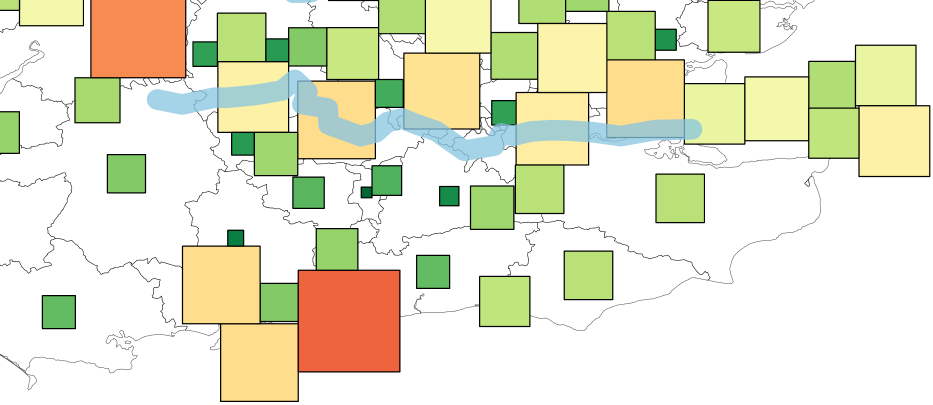
\includegraphics[width=\linewidth,keepaspectratio]{figure/cover.png}
    \caption{The River Thames passing through a cartographic representation of the NHS CCGs in London and surrounding areas.}
    \label{fig:cover}
\end{figure}

\end{samepage}

Among the four types of cartogram categorized in a survey by \citet{nusrat2016State} (See \Cref{sec:RelatedWork} for definitions of contiguous, non-contiguous, rectangular, and Dorling), a trade-off is made between types of accuracy (See \Cref{table:accuracy}).
For this project, we focus on non-contiguous cartograms like Demers cartograms because they facilitate statistical comparison between regions, they can make good use of screen space, and comparison of regions is useful when studying Electronic Health Records (EHR) data.
Demers cartograms offer the advantage in cases where the data is not directly correlated to region sizes. Also, the comparison of magnitudes becomes an area estimation task, which is more effective for a numeric data encoding \cite{munzner2014Visualization}.
Building on Demers cartograms \cite{ian2002Cartogram}, we introduce and develop novel features, such as rivers, aiming to improve the readability and geographical accuracy without sacrificing statistical accuracy.
Standard Demers cartograms are composed of square nodes. As such, this can reduce their legibility.
We implement a new hybrid cartographic layout algorithm that combines rivers with the placement of the nodes representing geo-referenced regions. 
We hypothesize that introducing rivers improves the overall legibility of a cartogram. 
By \textit{legibility} we mean readability and ability to interpret the cartogram.  
To assess this hypothesis, we designed an experimental setup where participants engaged in correspondence and location tasks as part of a user study.
To reduce error and make efficient use of screen space, the algorithm also updates the position of rivers to accommodate the node layout.
We then apply the algorithm to a real-world case study using EHR data to evaluate the result.
We present a user study that demonstrates its effectiveness.

Our contributions include:

\begin{itemize}
    \setlength\itemsep{0px}
    \item A new variant of Demers cartograms that incorporates rivers to improve readability and recognizability,
    \item A novel hybrid layout algorithm that combines node positions with features such as rivers,
    \item A user study evaluation of the technique with an application to EHRs.
\end{itemize}

The results of the user study indicate that rivers can improve the legibility of cartograms.
One of the major challenges involved is developing a layout algorithm that handles different shapes.
In other words, the hybrid layout algorithm is novel because it handles different types of elements: square representing regions and polylines representing rivers.
Another challenge we overcome in developing the algorithm is to resolve stalemate situations introduced by rivers while minimizing error.